
%(BEGIN_QUESTION)
% Copyright 2014, Tony R. Kuphaldt, released under the Creative Commons Attribution License (v 1.0)
% This means you may do almost anything with this work of mine, so long as you give me proper credit

Calculate the amount of voltage between point A and ground ($V_A$) given the component values shown:

$$\includegraphics[width=15.5cm]{i03049x01.eps}$$

State your answer both in symbolic form (e.g. ??? volts $\angle$ ?? degrees) as well as in a phasor diagram showing the source voltage (its phase angle assumed to be zero degrees) and $V_A$.

\underbar{file i03049}
%(END_QUESTION)





%(BEGIN_ANSWER)

\noindent
{\bf Partial answer:}

$$V_A = 8.588 \hbox{ V} \angle -54.87^o$$

Note how the voltage between point A and ground is actually {\it larger} than the transformer's output voltage of 5.5 volts!
 
%(END_ANSWER)





%(BEGIN_NOTES)

Source voltage in this circuit is the 110 VAC supply stepped down by a factor of 20, at a reference phase angle of zero degrees:

$${110 \hbox{ V} \angle 0^o \over 20} = 5.5 \hbox{ V} \angle 0^o$$

Since this is a series circuit, total impedance is the phasor sum of all component impedances:

$$Z_R = 2.2 \hbox{ k}\Omega \angle 0^o$$

$$Z_L = 2.827 \hbox{ k}\Omega \angle 90^o$$

$$Z_C = 2.653 \hbox{ k}\Omega \angle -90^o$$

$$Z_{total} = Z_R + Z_L + Z_C = 2.207 \hbox{ k}\Omega \angle 4.544^o$$

Current in this series circuit will be equal to source voltage divided by total impedance:

$$I = {5.5 \hbox{ V} \angle 0^o \over 2.207 \hbox{ k}\Omega \angle 4.544^o} = 2.492 \hbox{ mA} \angle -4.544^o$$

Multiplying this current by each of the impedances yields voltage drops for each component:

$$V_R = I Z_R = (2.492 \hbox{ mA} \angle -4.544^o)(2.2 \hbox{ k}\Omega \angle 0^o) = 5.483 \hbox{ V} \angle -4.544^o$$

$$V_L = I Z_L = (2.492 \hbox{ mA} \angle -4.544^o)(2.827 \hbox{ k}\Omega \angle 90^o) = 7.046 \hbox{ V} \angle 85.46^o$$

$$V_C = I Z_C = (2.492 \hbox{ mA} \angle -4.544^o)(2.653 \hbox{ k}\Omega \angle -90^o) = 6.611 \hbox{ V} \angle -94.544^o$$

The voltage between point A and ground will be equal to the sum of the capacitor and resistor voltage drops:

$$V_A = 6.611 \hbox{ V} \angle -94.544^o + 5.483 \hbox{ V} \angle -4.544^o = 8.588 \hbox{ V} \angle -54.87^o$$

A phasor diagram shows $V_A$ along with the phasor representing source voltage:

$$\includegraphics[width=15.5cm]{i03049x02.eps}$$

%INDEX% Electronics review: AC reactance and impedance
%INDEX% Electronics review, phasor expressions of circuit quantities
%INDEX% Electronics review: series and parallel AC circuits

%(END_NOTES)


